% !TEX root = ../thesis.tex
\chapter{Research: pureSVD strenght}
\label{chapter:<research_puresvd_strenght>}

\section{Introduction}
\label{sec:research_introduction}

This represents the research bla bla bla

\section{Sources}
\label{sec:research_sources}

For this research a number of different resources has been used in order to collect the maximum number of surveys with the minimum budget. Aside of Amazon Mechanical Turk of which we discussed on secion \ref{sec:crowdsourcing}, also Facebook and Google plus have been used in order to test if a survey can go viral on social networks.

In order to maximize the user attention a whiteboard rewarding an eligibility of prize to the ones that perform the survey has been used. The Facebook post that promoted one of the three surveys that have been performed is displayed in figure \ref{fig:facebook_survey}.

\begin{figure}
  \centering
  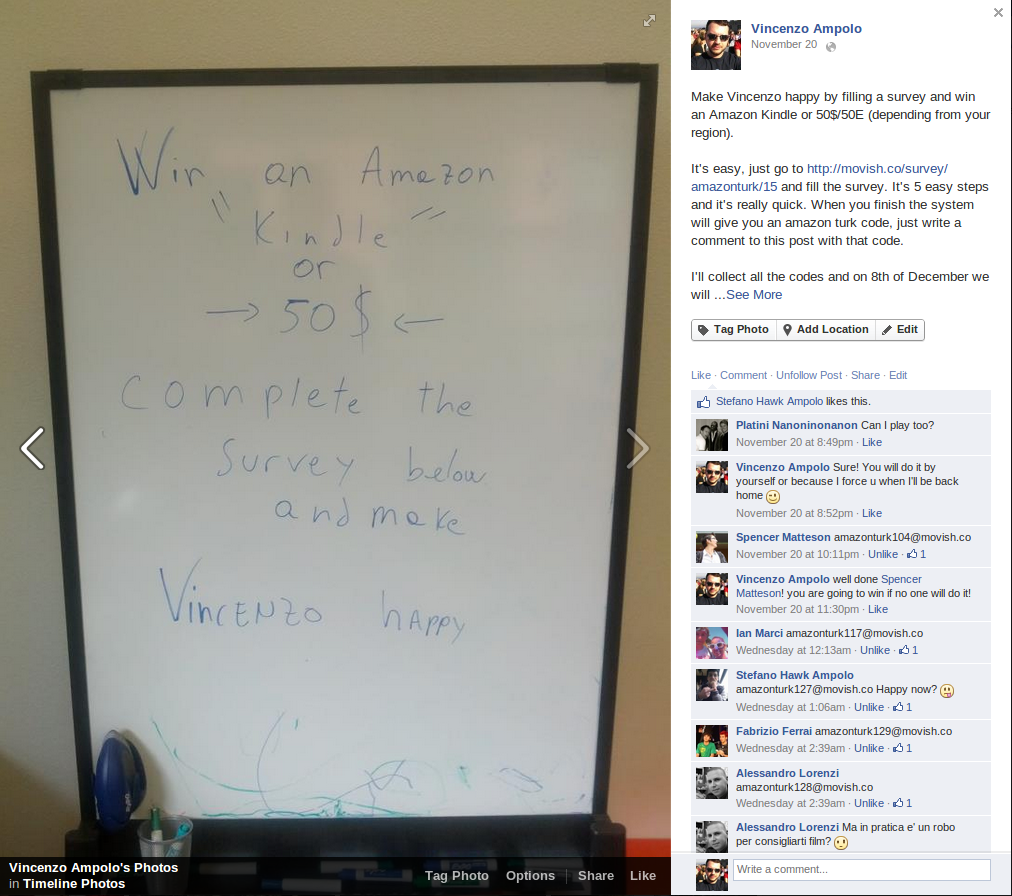
\includegraphics[width=\textwidth]{figures/facebook_survey.png}
  \caption{Facebook post to participate to a survey}
  \label{fig:facebook_survey}
\end{figure}

The whiteboard message is: \textit{Win an Amazon Kindle or \$50, complete the survey below and make Vincenzo happy}. The message had two goals: stimulate all my close friends in taking action in order to help me in my research and to stimulate all the not close friends in performing the survey due to the prize they could win. In order to be eligible for the prize the user/friend had to write the Amazon Mechanical Turk code that is displayed at the end of the survey as comment to the post.  The same message has been posted on Google plus and can be seen in figure \ref{fig:google_plus_survey}.

\begin{figure}
  \centering
  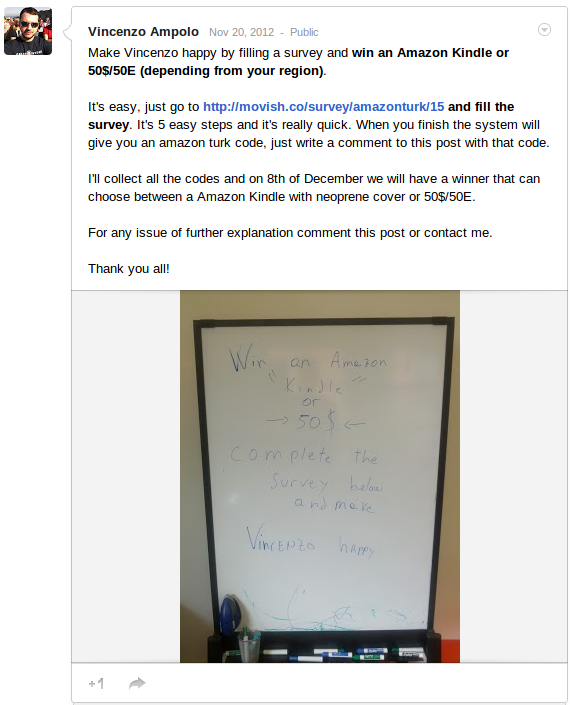
\includegraphics[width=\textwidth]{figures/google_plus_survey.png}
  \caption{Google plus post to participate to a survey}
  \label{fig:google_plus_survey}
\end{figure}

The facebook post was able to retrieve a total 13 users performing the survey of which 7 of them can be categorized as not close friends. The Google plus post wasn't able to stimulate any user.

\section{Survey}
\label{sec:research_survey}

In order to fulfill the goal of this research a survey type of \textbf{algorithm\_strength} with 5 free ratings using \textbf{pureSVD} algorithm has been chosen.

\begin{figure}
  \centering
  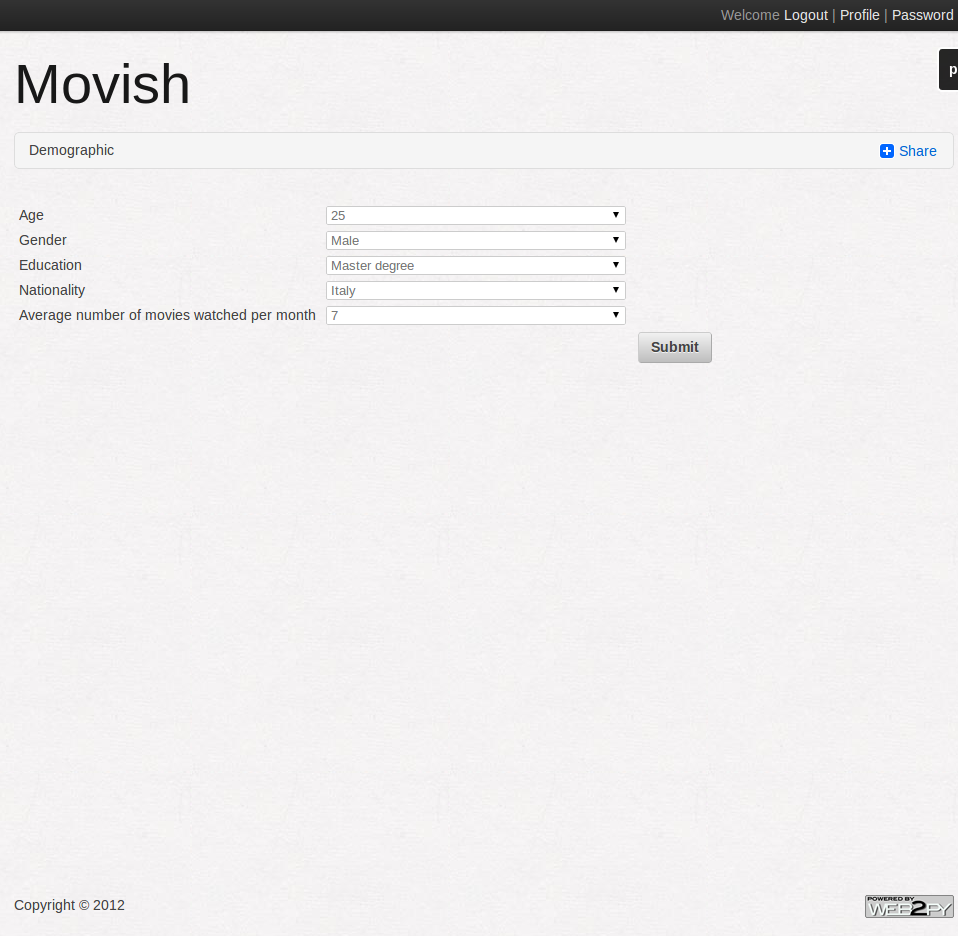
\includegraphics[width=\textwidth]{figures/survey_demographic.png}
  \caption{Survey phase 1}
  \label{fig:survey_phase_1}
\end{figure}

\begin{figure}
  \centering
  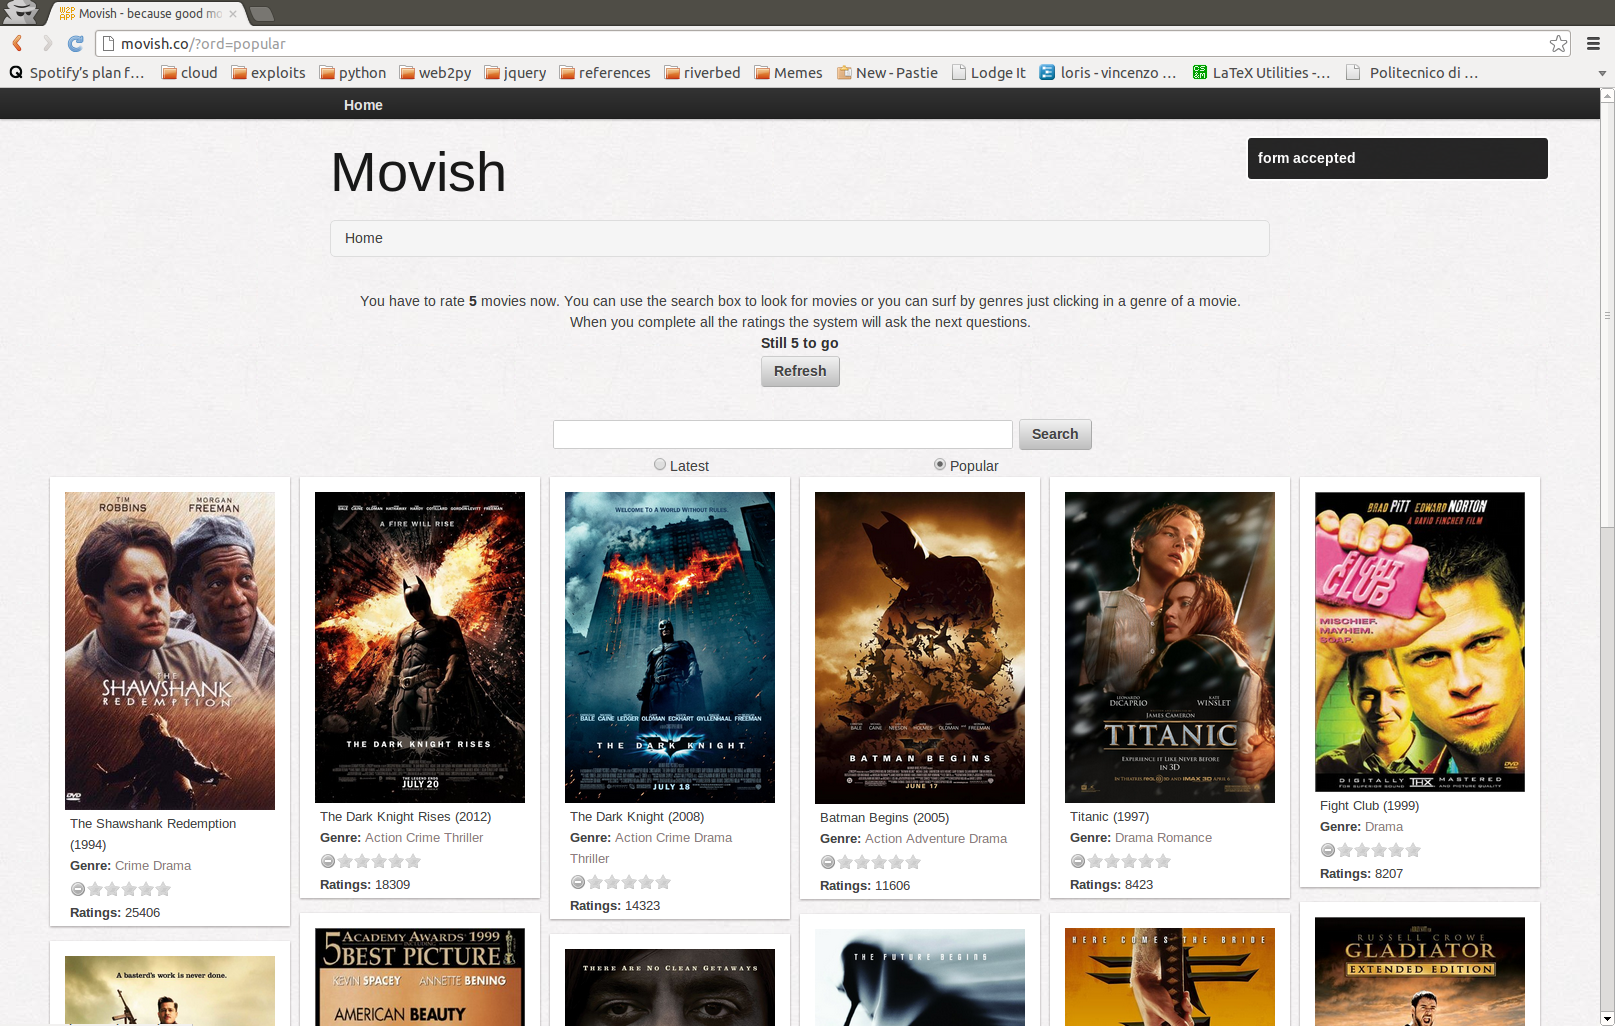
\includegraphics[width=\textwidth]{figures/free_ratings.png}
  \caption{Survey phase 2}
  \label{fig:survey_phase_2}
\end{figure}

\begin{figure}
  \centering
  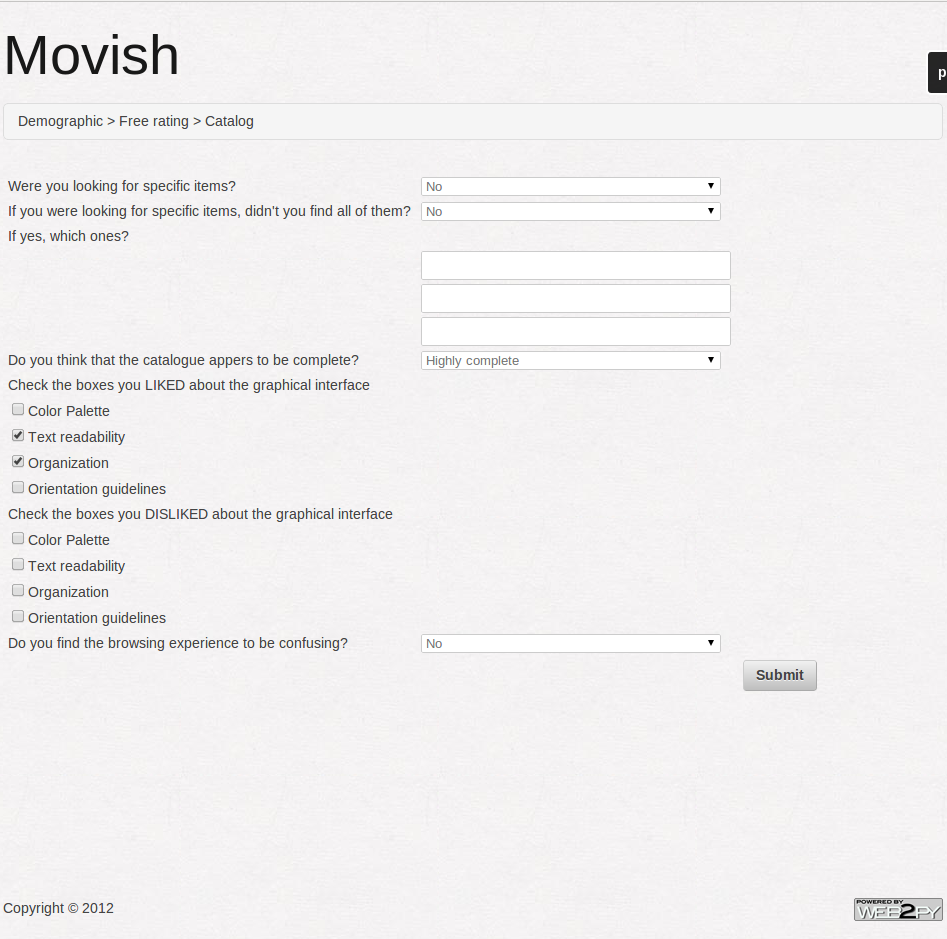
\includegraphics[width=\textwidth]{figures/survey_catalog.png}
  \caption{Survey phase 3}
  \label{fig:survey_phase_4}
\end{figure}

\begin{figure}
  \centering
  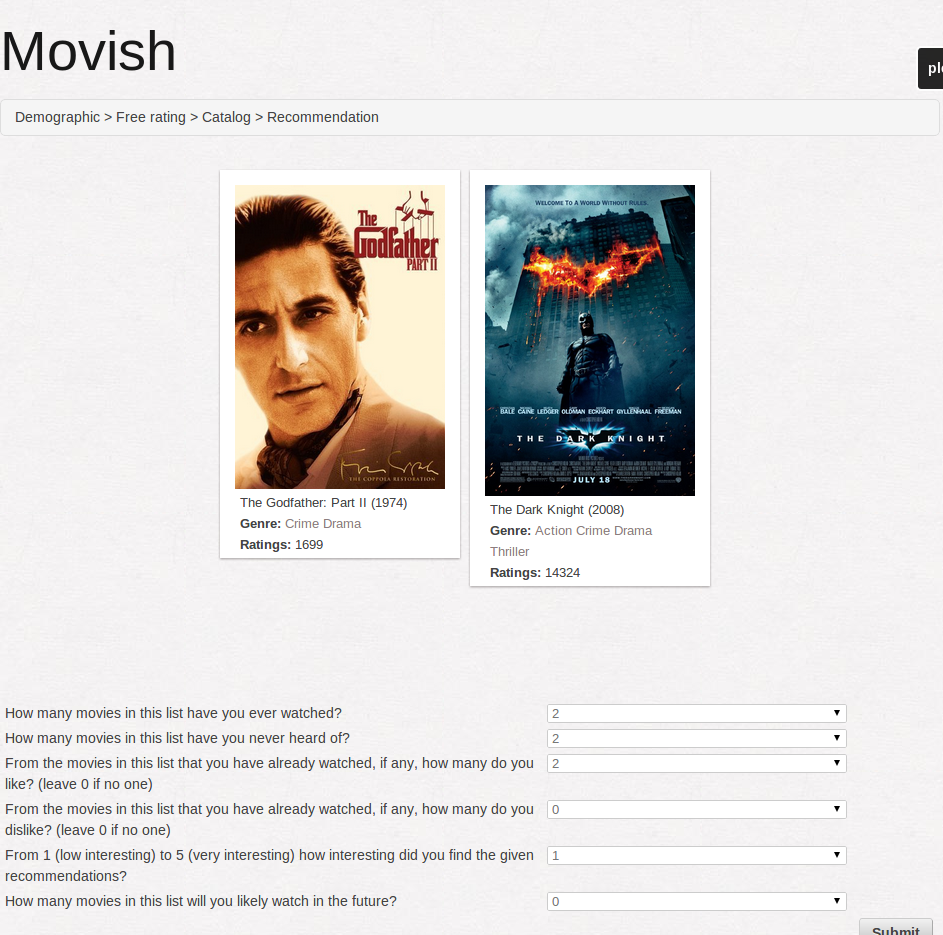
\includegraphics[width=\textwidth]{figures/survey_recommendation.png}
  \caption{Survey phase 4}
  \label{fig:survey_phase_4}
\end{figure}

\begin{figure}
  \centering
  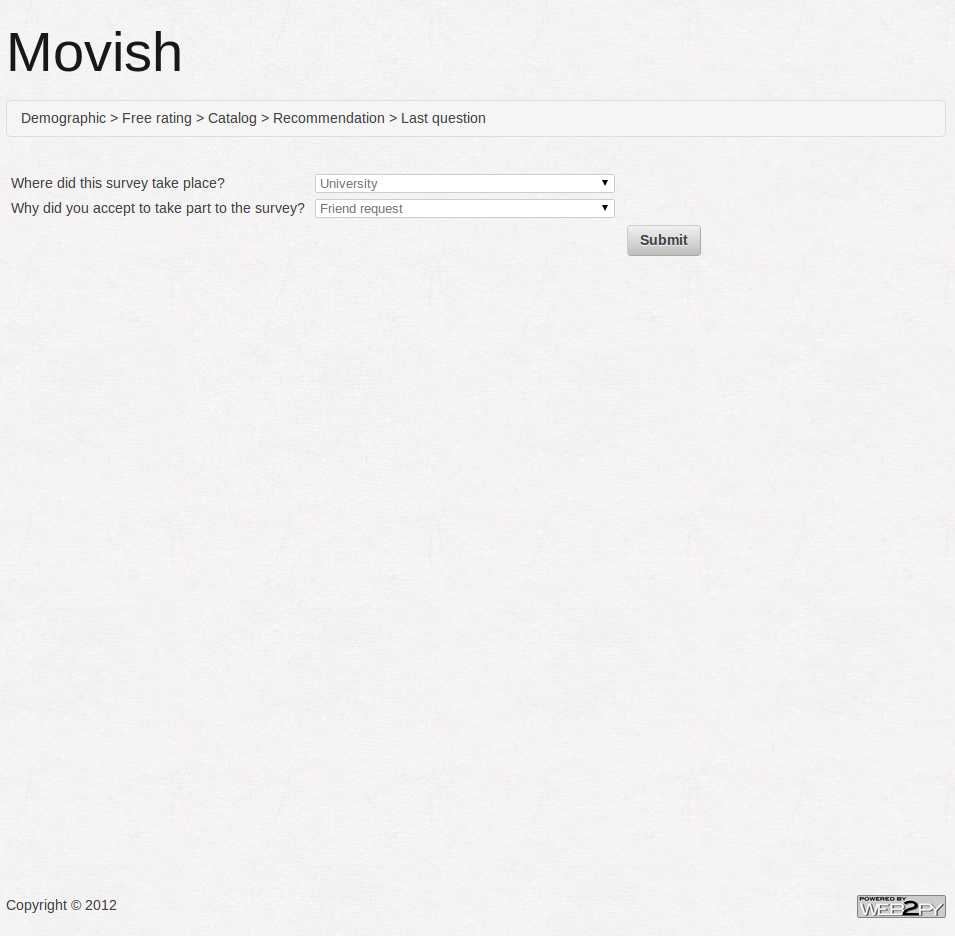
\includegraphics[width=\textwidth]{figures/survey_localinfo.png}
  \caption{Survey phase 5}
  \label{fig:survey_phase_5}
\end{figure}


\section{Analysis}
\label{sec:research_analysis}

\section{Conclusions}
\label{sec:research_conclusions}


\acresetall